\chapter{Theory and Method}

\section{Many Body Theory}


Many-body problems refer to systems
with many particles (many electrons, many atoms, many molecules, etc.), where there are interactions among them. Imagine that there is no interaction between particles. In that case, each particle is like an independent body, and there is no relation between all bodies in the system such that we can study the behaviour of each body independently. In fact, when there is no interaction, the problem of one many-body system changes to many one-body systems. Consequently, interactions are the basic part of many-body problems \cite{Richard}.

The importance of many-body problems raises from the fact that all of the real physical systems include particles. For instance, the interaction between nucleons in a nucleus is governed by the nuclear force, electrons in an atom or metal interact by Coulomb forces, and atoms are bonded together by electrostatic attraction. 




The many-body problem is one of the most challenging dilemmas in physics since there is complex motion of particles in an interacting system. In Fig.\ref{fig:particle} the behaviour non-interacting and interacting particles can be seen. Non-interacting particles have simple behaviour while interacting particles show complicated behaviour referred as emergent phenomena \cite{Eva}.


\begin{figure}[!htb]
  \includegraphics[width=0.5\linewidth]{fig2/non.pdf}
  \includegraphics[width=0.5\linewidth]{fig2/inter.pdf}
  \caption{Non- interacting and interacting particles.}
\label{fig:particle}
\end{figure}


\subsection{Green's Function}

The Green's function method has different applications in several fields of Physics, from classical differential equations to quantum many-body problems. For example, in the context of quantum mechanics, Green's functions are correlation functions, from which it is possible to extract some information such as the density of states, relaxation times and response functions from the system. Green's functions theory is a useful mathematical tool to deal with linear differential equations. These functions were named after physicist and mathematician George Green (1793-1841).The Green's functions were used as auxiliary functions for solving boundary-value problems. Moreover, a Green's function is a solution of a linear differential equation with a Dirac delta inhomogeneous source (sometimes referred as a delta or unit pulse) with homogeneous boundary conditions \cite{Mariana}.
Usually, the problems that we are dealing with are many body systems of quantum particles interacting with each other or with quantized versions of classical waves. To obtain physically relevant information about the properties of these interacting many-particle systems, the definition of the Green's functions should include all general cases\cite{Economou}. 

As mentioned above, Green's functions are the elementary response functions of a many-body system to an external force. The one- particle Green's function can be defined as\cite{Piers}:

\begin{equation}
    G_{\lambda\lambda'}(t-t')=-i \langle\phi|T\psi_\lambda(t)\psi_{\lambda'}^\dagger(t')|\phi\rangle
\end{equation}
In this equation $|\phi\rangle$ is the many-body ground state and  $\psi_\lambda(t)(\psi_{\lambda'}^\dagger(t'))$ are annihilation (creation) operators, $\lambda$ denotes the momentum and spin of the particle $\lambda \equiv P\sigma$, and

\begin{equation}
  T\psi_\lambda(t)\psi_{\lambda'}^\dagger(t')=\begin{cases}
    \psi_\lambda(t)\psi_{\lambda'}^\dagger(t')\hspace{1cm} (t>t')\\
    \pm\psi_{\lambda'}^\dagger(t')\psi_\lambda(t) \hspace{1cm} (t<t') \hspace{1cm} 
  \end{cases}
\end{equation}

\noindent represents the time-ordering for fermions and bosons ($-$ is used for Fermions and$+$ for Bosons). In fact, the time ordering operator takes products of operators, that each operator belongs to a specific time, and modifies the order of operators in a way that every operator has only later operators to its left and earlier operators to its right. Then

\begin{equation}
    G_{K\sigma,K',\sigma'}(t-t')=  \delta_{\sigma\sigma'}\delta_{KK'}G(K,t-t')
\end{equation}

\noindent is diagonal in $K$ and $K'$ (in the continuum limit $\delta_{KK'}$ is $(2\pi)^D\delta^{(D)}(K-K')$). Now we can write:

\begin{equation}
    G(K,t-t')= -i \langle\phi|T\psi_{K\sigma}(t)\psi_{K\sigma'}^\dagger(t')|\phi\rangle
\end{equation}

\noindent and in the space coordinate the Green's functions can be written as:

\begin{equation}
    G(X-X',t-t')= -i \langle\phi|T\psi_{\sigma}(X,t)\psi_{\sigma'}^\dagger(X',t')|\phi\rangle .
\end{equation}


By replacing $\psi(X,t)$ with $\int_K\psi_{K\sigma}e^{i(K.X)}$, it can be seen that the coordinate-space Green's function is equivalent to the Fourier transform of the momentum-space Green's function:
\begin{equation}
    G(X-X',t)= \int_{K,K'}e^{i(K.X-K'.X')}-i \langle\phi|T\psi_{K\sigma}(t)\psi_{K'\sigma}^\dagger(0)|\phi\rangle
    \label{eq:gg}
\end{equation}

\noindent where 

\begin{equation}
    -i \langle\phi|T\psi_{K\sigma}(t)\psi_{K'\sigma}^\dagger(0)|\phi\rangle= \delta_{KK'}G(K,t-t'),
\end{equation}

\noindent such that Eq (\ref{eq:gg}) reduces to:

\begin{equation}
     \int\frac{(d^3k)}{(2\pi)^3}G(K,t)e^{iK.(X-X')}
\end{equation}

The Fourier transform of this equation in the time domain is:

\begin{equation}
    G(K,t)=\int_{-\infty}^{\infty}\frac{d\omega}{2\pi}G(K,\omega)e^{-i\omega t} .
\end{equation}

\noindent In this equation $\omega$ is frequency and $G(K,\omega)$ is the frequency dependent Green's function:

\begin{equation}
    G(K,\omega)=\int_{-\infty}^{\infty} dtG(K,t)e^{-i\omega t} .
\end{equation}
Now we are in a position to relate the Green's function in coordinate space to its propagator:
\begin{equation}
    -i \langle\phi|T\psi_{\sigma}(X,t)\psi_{\sigma'}^\dagger(X',t')|\phi\rangle=\int \frac{d^3kd\omega}{(2\pi)^4}G(K,\omega)e^{i[K.(X-X')-\omega(t-t')]}
    \label{eq:sprop}
\end{equation}

\subsection{Green's function of free fermions}
Now we can calculate the Green's function of a degenerate Fermi liquid of non-interacting fermions in its ground state.  We use an interacting Hamiltonian which is in the Heisenberg representation:
\begin{equation}
    H=\hat{H_0}-\mu N=\sum_{\sigma}\epsilon_Kc_{K\sigma}^\dagger c_{K\sigma}.
\end{equation}
In this equation $\epsilon_K=\frac{\hbar^2k^2}{2m}-\mu$ and $c_{K \sigma}(c_{K \sigma}^\dagger)$ is the creation (annihilation) operator of fermions in momentum space. The wave function of the ground state for a fluid of fermions is:

\begin{equation}
    |\phi\rangle=\prod_{\sigma|K|<k_f}c_{K\sigma}^\dagger|0\rangle.
\end{equation}

\noindent In the Heisenberg picture, time propagation of the system $c_{K\sigma}^\dagger(t)=e^{i\epsilon_K t}c_{K\sigma}^\dagger , c_{K\sigma}(t)=e^{-i\epsilon_K t}c_{K\sigma}$. To go forward in the time domain, we are allowed to add a fermion above the Fermi energy, so:

\begin{equation}
\begin{split}
    \langle\phi|c_{K\sigma}(t)c_{K'\sigma'}^\dagger(t)|\phi\rangle&=\delta_{\sigma\sigma'}\delta_{KK'}e^{-i\epsilon_K(t-t')}\langle\phi|c_{K\sigma}c_{K'\sigma'}^\dagger|\phi\rangle\\
    &=\delta_{\sigma\sigma'}\delta_{KK'}(1-n_K)e^{-i\epsilon_K(t-t')}
    \end{split}
\end{equation}

\noindent In the last equation $n_K=\theta(|k_F|-|K|)$ is Heaviside step distribution. For backward time propagation we need to annihilate a fermion and create a hole beneath the Fermi energy, so:
\begin{equation}
    \langle\phi|c_{K'\sigma'}^\dagger(t)c_{K\sigma}(t)|\phi\rangle=\delta_{\sigma\sigma'}\delta_{KK'}n_Ke^{-i\epsilon_K(t-t')}
\end{equation}

\noindent then by using Eq. \ref{eq:sprop} we can find

\begin{equation}
    G(K,t)=-i[(1-n_K)\theta(t)-n_K\theta(-t)]e^{-i\epsilon_Kt}
\end{equation}

\noindent This equation can be expressed for two different situation:

\begin{equation}
    G(K,t)=\begin{cases}
    -i\theta_{|K|-|K_F|}e^{-i\epsilon_Kt}\hspace{1cm} (t>0)\hspace{1cm} particles\\
    i\theta_{|K_F|-|K|}e^{-i\epsilon_Kt}\hspace{1cm} (t<0)\hspace{1cm}holes: $particles moving backwards in time$
    \end{cases}
\end{equation}

Now we are in a place that we can find the Fourier transform of the free fermion's Green's function:

\begin{equation}
\begin{split}
    G(K,\omega)&=-i\int_{-\infty}^{\infty} dt e^{i(\omega-\epsilon_K)t} [\theta_{k-k_F}\theta(t)-\theta_{k_F-k}\theta(-t)] e^{-|t|\delta}\\
    &=-i\left[\frac{\theta_{k-k_F}}{\delta-i(\omega-\epsilon_K)}-\frac{\theta_{k_F-k}}{\delta+i(\omega-\epsilon_K)}\right]
\end{split}
\end{equation}

In this equation $e^{-|t|\delta}$ is called \emph{convergence factor}. We introduced this term to make the integrals converge, we use the $lim \: \delta \rightarrow 0^+$. Then the free fermion propagator can be written as 

\begin{equation}
    G(K,\omega)=\frac{1}{\omega-\epsilon_K+i\delta_K},
\end{equation}

\noindent where $\delta_K= \delta (sgn(k-k_F))$.







\section{Feynman Diagram}

Feynman diagrams are a powerful tool for quantum theory calculations. Richard P. Feynman introduced this method to explain quantum interactions \cite{David, James, Kaiser}.  
Feynman diagrams usually include all information about the diagrams and the process of constructing the mathematical expression of the diagrams. There are some specific rules for this method known as "Feynman rules". The solid straight lines introduce the fermions, wavy lines represent Bosons, and dots or vertices are for the coupling \cite{James, Kaiser}.


%\begin{figure}[ht]
%\centering
%    \includegraphics[width=0.25\linewidth]{fig2/line.pdf}
%    \includegraphics[width=0.25\linewidth]{fig2/wavy.pdf}
%\caption{solid line with an arrow
%pointing toward the vertex, and a phonon in the
%initial states is represented by a wavy line meeting a
%vertex
%\label{fig:feynman_diagram}}
%\end{figure}


By Wick's theorem\footnote{Wick's theorem is used to reduce a product of creation and annihilation operators as a sum of normally ordered terms.}, we can evaluate the exact Green's functions as a perturbation expansion involving expressions of free Green's functions $ G_{0}$ and the perturbation potential $ V$. That representation is equivalent to the Feynman diagram approach. The Feynman diagrams are a demonstrative way to solve the many-particle problems and the perturbation expansion of the Green's functions \cite{Andre, wick, WESTWANSKI}.


\begin{figure}[ht]
\centering
    \includegraphics[width=0.40\linewidth]{fig2/full_green.pdf} 
    
    
    \includegraphics[width=0.40\linewidth]{fig2/free_green.pdf}
    
    
    \includegraphics[width=0.30\linewidth]{fig2/po.png}
\caption{Feynman Diagram of Full Green's function, free Green's function and Coulomb interaction, respectively. 
\label{fig:green_diagram}}
\end{figure}

Shown in Fig. \ref{fig:green_diagram}, the Green's function can be represented as the creation of a particle at $(r', t')$ then it will propagate to the point $(r, t)$ where the particle is annihilated. In the Feynman diagram representation, the full Green's function is shown by a double line joining these two points, and the free Green's function is described by a single line. Also, the Coulomb potential is drawn by a wavy line, at the vertex, the momentum and energy are conserved \cite{Sam, Strohm}.

\subsection{Self- Energy}


The feedback of the interacting environment on a propagating particle can be understood by the concept of self-energy \cite{Piers}. The self-energy $\Sigma(\overrightarrow{k},\omega)$ can be found as the sum of all diagrams that cannot be broken into two by breaking a single internal fermion line(The left arm and right arm are electron lines in a diagram which are called external, and all other electron lines are called internal). It should be mentioned that in the self-energy diagrams there must be a momentum $\overrightarrow{k}$ and energy $\omega$ coming in and going out. But the Green function lines that carry this energy and momentum to the vertices are not included \cite{Sam, Richard}. Some examples of irreducible diagram is shown in Fig. \ref{fig:irreducible} \cite{Richard}. It is clear that by cutting a Fermion line, we can not find a new diagram.
 
 
 \begin{figure}[ht]
\centering
    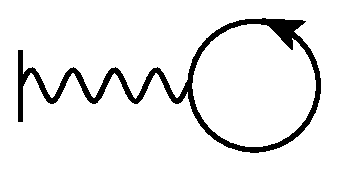
\includegraphics[width=0.17\linewidth]{fig2/irreduc1.eps}
    \includegraphics[width=0.17\linewidth]{fig2/irreduc2.eps}
    \includegraphics[width=0.17\linewidth]{fig2/irreduc3.eps}
    \includegraphics[width=0.17\linewidth]{fig2/irreduc4.eps}
\caption{Diagrammatic representation Feynman diagrams introducing the irreducible self-energy $\sum^{(i)}=(k, \omega).$
\label{fig:irreducible}}
\end{figure}
 
 
 If a diagram is not irreducible or on the other hand it can be separated, it is called reducible and it's a part of the Green's function. some examples can be seen in Fig. \ref{fig:reducible} \cite{Richard}:
 
 
 \begin{figure}[ht]
\centering
    \includegraphics[width=0.17\linewidth]{fig2/reduc1.eps}
    \includegraphics[width=0.17\linewidth]{fig2/reduc2.eps}
\caption{Diagrammatic representation Feynman diagrams introducing the reducible self-energy $\sum$.
\label{fig:reducible}}
\end{figure}


Now we are in a position that we can define a mathematical expression for the self-energy diagram by using the Feynman rules, as we know the self-energy is the sum of all irreducible Feynman diagrams. It is the same as that of the irreducible diagram it was constructed from except the external lines of $G_0(k, \omega)$ \cite{Dimitri}. 

\begin{equation}
    \Sigma (k)= \sum_i \Sigma^{(i)}(k)
\end{equation}

Now we can show that the particle propagator can be extended as self-energy series in Fig. \ref{fig:GREEN_expand} \cite{Piers,MICHAEL}:

\begin{figure}[ht]
\centering
    \includegraphics[width=0.9\linewidth]{fig2/GREEN.eps}
    \caption{Green's function as expansion of self-energy series.}
\label{fig:GREEN_expand}
\end{figure}

\noindent This graphical expansion can be written in mathematical language as:

\begin{equation} \label{eq:green_expand}
    G(k,\omega) = \frac{G_0(k,\omega)}{1-\Sigma(k,\omega) G_0(k,\omega)}= \frac{1}{(G_0(k, \omega))^{-1}-\Sigma (k,\omega)}
\end{equation}

\noindent then Eq. \ref{eq:green_expand} can be written as:

\begin{equation}
    G(k, \omega)= \frac{1}{\omega - \epsilon_k - \sum (k, \omega)+i\delta}.
\end{equation}

\noindent This equation is known as the Dyson equation. Now we can see that the full Green's function is determined by the Dyson equation \cite{Piers, MICHAEL}.

\begin{figure}[ht]
\centering
    \includegraphics[width=0.9\linewidth]{fig2/dyson.eps}
     \caption{Schematical representation of full Green's function. The full Green's function can be obtained by using the Dyson equation.}
\label{fig:dyson}
\end{figure}

The equation we represented in Fig. \ref{fig:dyson} is called Dyson equation. Physically, the self-energy which is a complex function $(Re+iIm)$ represents the cloud of particle-hole excitations which follow the propagating electron, "dressing" it into a quasiparticle \cite{Ivanov, Andre, Piers}. 






\section{Anderson Impurity Model}

The Anderson impurity model was originally introduced by Anderson in the 1961 to describe the behaviour of magnetic impurities (Fe, Mn, Cr) diluted into non-magnetic metals \cite{Anderson}.  In those systems, an anomalous minimum in the electrical resistivity at low temperatures was seen, for which the interaction of impurities and the conduction electrons seems to have caused this phenomenon \cite{Haas}. The impurity Anderson model maps a lattice site of interacting electrons onto a mean-field approximation. In the lattice problem, the electrons repulse each other via the on-site Coulomb repulsion $U$, and they can move in the lattice sites by the hopping parameter $t$  \cite{Anderson}. In Fig. \ref{fig:bath} schematical representation of Anderson impurity model has been shown.


\begin{figure}[ht]
\centering
    \includegraphics[width=0.6\linewidth]{fig2/bath1.pdf}
   
\caption{The impurity Anderson model maps the physics of interacting electrons on a lattice onto a mean-field approximation. In the lattice problem, the electrons repulse each other via the on-site Coulomb repulsion $U$, and they can move in the lattice sites based on the hopping parameter $t$.}
\label{fig:bath}
\end{figure}

The Anderson model is an important ingredient of the dynamical mean field theory for correlated lattice models, which will be further discussed. The Hamiltonian of the Single Impurity Anderson Model (SIAM) includes three different parts \cite{Carlos}:   

\begin{equation}
H_A=H_a+H_b+H_h
\end{equation}

\noindent where the second term

\begin{equation}
    H_b=\sum_k\epsilon_kc_{k\sigma}^{\dagger} c_{k\sigma}
\end{equation}

\noindent Here $\epsilon_k$ is the energy of electron in the conduction band and it is measured from the Fermi energy, $c_{k\sigma}^{\dagger}$ and $c_{k\sigma}$ are creation and annihilation operators and $\sigma$ describes spin. The first term is

\begin{equation}
    H_a=\epsilon_d n_d+Un_{d\uparrow}n_{d\downarrow},
\end{equation}

\noindent describes the interacting electron level, where $\epsilon_d$ is the energy of electrons in the localized impurity state, the total occupancy of the impurity level is $n_d=n_{d\uparrow}+n_{d\downarrow}$, and $U>0$ represents the Coulomb repulsion between a pair of localized electrons. Finally, the last term is

\begin{equation} \label{eq:hyb}
    H_h=\sum_k \frac{t_k}{\sqrt{N_0}}(c_{k\sigma}^\dagger d_\sigma+H.c.).
\end{equation} 

Where the number of unit cells in the host is given by $N_0$, $t_k$ is  the
hybridization matrix elements,and $H.c$ introduces the hermitian conjugate.. 






In Eq. \ref{eq:hyb} we replace $V_k= \frac{t_k}{\sqrt{N_0}}$, and introduce the hybridization function $\Delta (\omega)$ which is the coupling of the impurity to the band \cite{Alexander}:

\begin{equation}
    \Delta (\omega)=\sum_{k \sigma}\frac{|V_k|^2}{\omega- \tilde{\epsilon_k}}
\end{equation}

\noindent The local free Green's function can be express as:

\begin{equation}
    \mathcal{G}_0^{-1}(\omega)\equiv \omega + \mu-\Delta(\omega)
\end{equation}

\noindent The interacting Anderson Green's function will be: 

\begin{equation} \label{eq:green_anderson}
    G_{A} =\frac{1}{\omega + \mu-\Delta(\omega)-\sum(\omega)}
\end{equation}

\noindent In the Eq. \ref{eq:green_anderson} the $\sum(\omega)$ is self- energy. 

\section{DMFT-impurity solver}

The dynamical mean-field theory was introduced by Metzner and Vollhardt in 1989 \cite{Walter}. It has become one of the most important tools for the study of strongly correlated electrons systems. The mean-field theory replaces a lattice problem with many degrees of freedom by a single-site effective problem with fewer degrees of freedom \cite{Antoine}. It has been shown that the Hubbard model could be mapped exactly to the Anderson impurity model in the limit of infinite coordination number \footnote{The number of ions, molecules or atoms which surround the central ion, molecule or atom is called Coordination number.} \cite{Walter}. In the interacting lattice, one site is chosen, and all other sites are mapped into a bath. Therefore, the lattice model is mapped to an "impurity" model that includes one single interacting site ("impurity"), which is coupled to the non-interacting bath \cite{Antoine}.


Electrons in a crystals lattices of finite dimension can leave a site by hopping to a neighbouring site. It also can return to the original site by just hopping backward, or in a complicated way, by hopping around a loop to get to the original site. The easiest problem to solve is the Bethe lattice \footnote{A Bethe lattice is an infinite connected node that each node is connected to z coordination number.} since there are no loop paths, it means if an electron hops off of a site, it can only return to the original site by reversing its path. In the DMFT when the number of neighbours $N$ increases, the probability of returning the electron to the original site by another paths decreases. Therefore, when $N=\infty$ it becomes impossible, by increasing N the mean field theory becomes an exact theory \cite{Mahan}. Dynamical mean-field theory (DMFT) maps the lattice of atoms and electrons to a single impurity atom and a bath of electrons this process is shown in  Fig.\ref{fig:mean_field}. Over time a lattice site can be unoccupied, occupied or doubly occupied by electrons. Impurity and bath are coupled together.



\begin{figure}[ht]
\centering
    \includegraphics[width=1 \linewidth]{fig2/mean_field.pdf}
     
\caption{ Dynamical mean-field theory (DMFT) maps the full lattice of atoms and electrons with a single impurity atom in a bath of electrons. Over time a lattice site can be unoccupied, occupied or doubly occupied by electrons. These dynamical processes, which results in time-resolved electron- electron interactions are taken into account in DMFT. Taken from ref \cite{Gabriel} with permission. \label{fig:mean_field}}
\end{figure} 


The lattice model we study is the Hubbard model, and it will be mapped to an Anderson impurity model (AIM) and we will use the DMFT self-consistency loop which is shown in Fig.\ref{fig:diagram} \cite{Antoine}. We can write the self-consistency loop as Fig.\ref{fig:diagram}: 

\begin{figure}[ht]
\centering
    \includegraphics[width=0.6 \linewidth]{fig2/diagram-crop.pdf}
     \caption{ The iterative self-consistent loop of Dynamical Mean-field theory. By repeated iterations, a self-consistent solution will be found.}
 \label{fig:diagram}
\end{figure} 

In the first step, we start from the solution of the Anderson Impurity Model (AIM), the self-energy $\sum (\omega)$. Then, we assume that the lattice self-energy is local, it means that lattice self-energy is k-independent and can be set equal to the self-energy of the impurity (DMFT approximation), $\sum_{Lat}(K,\omega) 	\approx \sum (\omega)$\cite{Antoine}. Therefore, the lattice Green's function can be express as:

\begin{equation}
    G_{Lat} (\omega) \equiv G_{Lat} (X=0, \omega) = \sum _K e^{iXK} G_{Lat} (K,\omega) = \int d\epsilon \frac{\rho (\epsilon)}{\omega+\mu-\epsilon-\sum(\omega)}.
    \label{eq:G_lat}
\end{equation}

In Eq.\ref{eq:G_lat}, $\rho (\epsilon) = \sum_{K} \delta (\epsilon - \epsilon_{K})$ is the density states of the band. The self-consistency condition forces the impurity and the lattice Green's functions to be equal $G_{Lat}= G_A $, 
which is equivalent to the mapping of the lattice to the impurity model. Then we can write the self-consistency equation as:

\begin{equation}
    G_{Lat}^{-1} (\omega) = \mathcal{G}_0^{-1}(\omega) -\sum (\omega).
    \label{eq:G_impurity}
\end{equation}

The free Green's function of the impurity model $\mathcal{G}_0(\omega)$ includes all the information of the bath of the single site. By using Eq. \ref{eq:G_impurity}, the bath of the Anderson impurity model $(\mathcal{G}_0(\omega))$, can be computed with $(G_{Lat})$ and $(\sum)$. Finally, $\sum (\omega)$ will be calculated in the last step, these steps and loop can be seen in Fig. \ref{fig:diagram}. Thus the loop is closed, and by repeated iterations, a self-consistent solution will be found. The steps that we mentioned above can be listed as below: 
\begin{itemize}
    \item Start with arbitrary self-energy $\sum (\omega)$.
    \item Find the lattice Green's function from Eq. \ref{eq:G_lat}.
    \item Find the dynamical mean-field $(\mathcal{G}_0(\omega))$ from Eq. \ref{eq:G_impurity}. 
    \item Use the dynamical mean-field impurity solver to find the new Green's function.
    \item By replacing new Green's function in Eq. \ref{eq:G_impurity} the self-energy can be found.
    \item These steps will continue until the self-energy converge.
\end{itemize}

\section{Continuous Time Auxiliary Field (CT-AUX) algorithm}


The central numerical effort in solving the dynamical mean field problems is solving the quantum impurity problem, by finding a self-energy for a specific Green's function. In this section we introduce the Continuous Time Auxiliary Field (CT-AUX) algorithm that we used as the DMFT impurity solver. Continuous-time quantum Monte Carlo (CT-QMC) is a method for solving the Anderson impurity model at finite temperature \cite{Hanna, werner, Joseph, staar}. In this approach, in the first step, the full partition function will be expanded as a series of Feynman diagrams, then employ Wick's theorem to group diagrams into determinants, and in the last step the Markov chain Monte Carlo will be used to add the resulting series \cite{werner}. 

The Hamiltonian of an extended Hubbard model on a two-dimensional square lattice is introduced below, we have divided the Hamiltonian into two parts,
interacting part, $H_{int}$, and non-interacting part, $H_0$ given by
 \cite{Hanna}:

\begin{equation}
    H=H_0+H_{int},
\end{equation}
\begin{equation}
    H_0=-\sum _{ij\sigma}t_{ij}(c_i ^ \dagger c_j + h.c.) -\mu \sum _{i\sigma} n_{i\sigma}+ \frac{K}{\beta},
\end{equation}
\begin{equation}
    H_{int}=\frac{1}{2} \sum _{ij\sigma \sigma^ \prime} U_{ij}^{\sigma \sigma^ \prime} (n_{i \sigma}n_{j\sigma^\prime} - \frac {n_{i \sigma}+n_{j\sigma^\prime}}{2}) - \frac{K}{\beta},
\end{equation}

As we described the Hubbard model before we know that the parameters $t, \mu$ and $U_{ij}^{\sigma \sigma^ \prime} $ stand for, electrons hopping between lattice sites, the chemical potential, and the density-density interactions between electrons, respectively. Moreover, we restrict that  electrons can only hop between nearest neighbour sites. The constant $\frac{K}{\beta}$ has been added to the Hamiltonians for simplicity in calculations in the next steps \cite{werner}. The interacting energy $U$ is defined as \cite{Hanna}:

\begin{equation}
   U_{ij}^{\sigma \sigma^ \prime}= \begin{cases} 
   U\delta_{ij} \delta _{\sigma - \sigma '}\\
   0 \delta_{ij} \delta _{\sigma \sigma '},
   \end{cases}
   \label{eq:U}
\end{equation}

\noindent In this equation, the interacting energy would be $U$ if $i=j$ and $\sigma=-\sigma'$, otherwise, it would be zero. We have Eq.\ref{eq:U} to the Hubbard interaction, which is a repulsive interaction for two electrons on the same site $i=j$ and with opposite spins $\sigma=-\sigma'$.  

The essential part of the partition function is the Hamiltonian. Therefore, when the Hamiltonian for a system is defined, it's easy to write the partition function, \cite{werner} 

\begin{equation}
    Z= Tr  e^{-\beta H}= Tr \: e^{-\beta (H_0 +H_{int})}.
\end{equation}

\noindent In the interaction representation the partition function can be written as 

\begin{equation}
    Z= Tr \left[e^{-\beta H_0} T_{\tau}  \: e^{-\int _0 ^{\beta} d \tau H U(\tau)}\right], 
    \label{eq: partition}
\end{equation}

\noindent In Eq. \ref{eq: partition} $T_{\tau}$ represents time ordering. After expanding the exponential part of partition function, Eq. \ref{eq: partition} will change to:

\begin{equation}
    Z= \sum _{k=0}^\infty \int_0 ^\beta d\tau _1 ... \int _{\tau _{k-1}} Tr \left[e^{-\beta H_0} e^ {\tau _k H_0} \: (-H_{int})... e^{-(\tau _2 - \tau _1)H_0} \: (-H_{int}) e^{-\tau _1 H_0}\right]
\end{equation}

\noindent where $0<\tau<\beta$ and $\tau$ displays imaginary time, also $H_{int}$ is: 

\begin{equation}
    -H_{int}= \left(\frac{K}{4\beta N_c ^2}\right) \sum _{ij \sigma \sigma'} \left(\frac{1}{2} \sum _{s=\pm 1} e^{\gamma _{ij} ^{\sigma \sigma'} s(n_{i\sigma}- n_{j\sigma'})}\right)
\end{equation}

\noindent $N_c$ represents the number of cluster sites and $n_{i \sigma}$ only can take the values zero or one, so it shows the possible occupations of site $i$. In 2D Hubbard model $\gamma _{ij} ^{\sigma \sigma'}$ is defined as:

\begin{equation}
    \cosh(\gamma _{ij} ^{\sigma \sigma'})= \begin{cases}
    1+\frac{\beta N_c ^2 U}{K} \quad i=j, \quad \sigma = -\sigma ' \\
    1  \qquad otherwise
    \end{cases}
    \label{eq:potential}
\end{equation}

\noindent Then we replace Eq. \ref{eq:potential} in the partition function equation:

\begin{equation}
    Z= \sum _{k=0} ^ {\infty} \: \sum _{\substack{s_l=\pm 1 \\ l=1,... ,k}} \sum _{\substack{i_l,j_l,\sigma _l, \sigma '_l \\ l=1,... ,k}} \int _0 ^ {\beta} d\tau _1 ... \int _{\tau _{k-1}} ^{\beta} \left(\frac{K}{8 \beta N_c ^2}\right)^2 \: Z_k ({s_l, \tau _l , i_l, j_l, \sigma _l, \sigma '_l})
\end{equation}

\noindent In this equation $Z_k$ is:

\begin{equation}
\begin{split}
    Z_k ({s_l, \tau _l , i_l, j_l, \sigma _l, \sigma '_l}) &= Tr [e^{-\beta H_0} \Pi _{l=k}^1 e^{\tau _l H_0} (e^{\gamma _{i_l j_l}^{\sigma _l \sigma '_l} s_l}- (e^{\gamma _{i_l j_l}^{\sigma _l \sigma '_l}} -1) c_{i_l \sigma _l} c_{i_l \sigma _l} ^ \dagger)\\
    & \times ((e^{-\gamma _{i_l j_l}^{\sigma _l \sigma '_l} s_l}- (e^{-\gamma _{i_l j_l}^{\sigma _l \sigma '_l}} -1) c_{j_l \sigma ' _l} c_{j_l \sigma ' _l} ^ \dagger) e^{-\tau _l H_0}]
    \end{split}
\end{equation}

We can write the partition function as a determinant of a $2k$ by $2k$ matrix $N^{2k}$ as below \cite {Hanna, Haule, werner}:

\begin{equation}
    Z_k({s_l, \tau _l , i_l, j_l, \sigma _l, \sigma '_l})= det [(N^{2k})_{ij\sigma\sigma'}^{-1}]
\end{equation}
\noindent where

\begin{equation}
    (N^{2k})_{ij\sigma\sigma'}^{-1}\equiv e^{V_{ij}^{\sigma\sigma'}}-G_{0\sigma\sigma'}^{ij}(e^{V_{ij}^{\sigma\sigma'}}-I)
\end{equation}

\noindent and

\begin{equation}
    e^{V_{ij}^{\sigma\sigma'}} \equiv diag \footnote{Diagonal terms of matrix.} (e^{-\gamma _{i_1 j_1}^{\sigma _1 \sigma '_1} s_1}, ..., e^{-\gamma _{i_n j_n}^{\sigma _n \sigma '_n} s_n})
\end{equation}

In case the spin arguments are unequal the Green's functions would be zero, so our matrix can be block diagonalized into spin up and spin down parts. cosequently, the partition function can be rewritten as:

\begin{equation}
    Z= \sum _{k=0} ^ {\infty} \: \sum _{\substack{s_l=\pm 1 \\ l=1,... ,k}} \sum _{\substack{i_l,j_l,\sigma _l, \sigma '_l \\ l=1,... ,k}} \int _0 ^ {\beta} d\tau _1 ... \int _{\tau _{k-1}} ^{\beta} \left(\frac{K}{8 \beta N_c ^2}\right)^2 \: det \left[(N_{\uparrow}^{(n)})^{-1}\right]\: det \left[(N_{\downarrow}^{(m)})^{-1}\right]
\end{equation}

To find the partition function we have to sample these series Quantum Monte Carlo methods. All possible configurations have to be sampled, and each configuration is a set of vertices. Each vertex can be described by  the spin, sites, auxiliary spin, and imaginary time indices. After sampling partition functions we can find the interacting Green's function.

\section{ Susceptibility and Inversion of Bethe-Salpeter Equation}

In this section, we explain how to calculate the generalized dynamical susceptibility. We use Refs. \cite{Thomas, Valli, Macridin} as our main references. First, we need to define the one-particle and two-particle Green's function in imaginary time $(\tau)$ \cite{Valli}:

\begin{equation}
    G_\sigma (\tau _1 ,\tau _2)= <T_\tau (c_{\sigma_1}^\dagger (\tau_1) c_{\sigma_2} (\tau_2))>,
\end{equation}
\begin{equation}
    G_{2,\sigma_1 \sigma_2 \sigma_3 \sigma_4} (\tau_1 , ...,\tau_4)= <T_\tau (c_{ \sigma_1}^\dagger (\tau_1) c_{\sigma_2} (\tau_2)c_{ \sigma_3}^\dagger (\tau_3) c_{ \sigma_4} (\tau_4))>.
\end{equation}

\noindent Where $T$ is time-ordering operator, $c^\dagger (c)$ creates (annihilates) an electron with spin $\sigma$. We can define generalized susceptibility in imaginary time by using one-particle Green's function  and two-particle Green's functions as follows:


\begin{equation}
     \chi _{\sigma_1 \sigma_2 \sigma_3 \sigma_4} (\tau_1 , \tau_2, \tau_3, \tau_4)= G_{2,\sigma_1 \sigma_2 \sigma_3 \sigma_4} (\tau_1 , ...,\tau_4)- G_{\sigma _1 \sigma _2}(\tau_1 , \tau _2) G_{\sigma _3 \sigma _4}(\tau_3 , \tau _4)
\end{equation}


\noindent we can confine the problem to only three-time arguments $\tau_1, \tau_2, \tau_3$ and consider $\tau_4=0$. Then the susceptibility would be:

\begin{equation}
    \chi _{\sigma_1 \sigma_2 \sigma_3 \sigma_4} (\tau_1 , \tau_2, \tau_3)= G_{2,\sigma_1 \sigma_2 \sigma_3 \sigma_4} (\tau_1 ,\tau_2, \tau_3,0)- G_{\sigma _1 \sigma _2}(\tau_1 , \tau _2) G_{\sigma _3 \sigma _4}(\tau_3 , 0).
\end{equation}


\noindent Moreover, by considering all symmetries we can define these spin combinations for susceptibility:

\begin{equation}
    \chi_{\sigma \sigma'}(\tau_1 , \tau_2, \tau_3)= \chi_{\sigma \sigma \sigma ' \sigma '}(\tau_1 , \tau_2, \tau_3) 
\end{equation}
\begin{equation}
    \chi_{\overline{\sigma \sigma'}}(\tau_1 , \tau_2, \tau_3)= \chi_{\sigma \sigma ' \sigma ' \sigma}(\tau_1 , \tau_2, \tau_3) 
\end{equation}

\begin{figure}[ht]
\centering
    \includegraphics[width=0.5\linewidth]{fig2/ph.pdf}
\caption{Particle-hole scattering. Taken from Ref \cite{Valli} with permission. \label{fig:ph}}
\end{figure}
\begin{figure}[ht]
\centering
    \includegraphics[width=0.55\linewidth]{fig2/pp.pdf}
\caption{Particle-Particle scattering. Taken from Ref \cite{Valli} with permission. \label{fig:pp}}
\end{figure}



The susceptibility equation can be expressed in frequency space via the Fourier transform. In this space, there are two different representations, particle-hole $(ph)$ and particle-particle $(pp)$. Using frequency space has two main reasons. First, In the $ph$ case, consider the scattering process of a hole with energy $- \nu$ and an electron with energy $\nu + \omega$, in this process the total energy is $\omega$ (this process is shown in Fig. \ref{fig:ph}). Second, In Fig. \ref{fig:pp} the $pp$ case, we look at the scattering of two electrons with energies $\nu$ and $\omega - \nu $. Again the total scattering energy will be $\omega$. The expression for particle-hole $(ph)$ and particle-particle $(pp)$ susceptibilities are  \cite{Valli, Macridin}:

\begin{equation}
    \chi_{ph \sigma \sigma'}^{\omega \omega ' \Omega} (k,k',q)= \int _{0}^\beta d\tau_1 d\tau_2 d\tau_3 \chi _{\sigma \sigma '}(\tau_1, \tau_2, \tau_3) \times e^{-i\omega \tau_1} e^{i(\omega + \Omega)\tau_2} e^{-i(\omega ' + \Omega)\tau_3}
    \label{eq:ph}
\end{equation}

where in this equation $d\tau_1 d\tau_2 d\tau_3 \chi _{\sigma \sigma '}(\tau_1, \tau_2, \tau_3)$  indicates outgoing electrons, and $e^{-i\omega \tau_1} e^{i(\omega + \Omega)\tau_2} e^{-i(\omega ' + \Omega)\tau_3}$ describes incoming electrons.

\begin{equation}
    \chi_{pp \sigma \sigma'}^{\omega \omega ' \Omega} (k,k',q)= \int _{0}^\beta d\tau_1 d\tau_2 d\tau_3 \chi _{\sigma \sigma '}(\tau_1, \tau_2, \tau_3) \times e^{-i\omega \tau_1} e^{i(\Omega - \omega ')\tau_2} e^{-i(\Omega- \omega)\tau_3}
    \label{eq:pp}
\end{equation}
 
In Eq.\ref{eq:ph} and \ref{eq:pp} $\omega$ and $\omega '$ are Fermionic frequencies $(\frac{(2n+1)\pi}{\beta})$, $\Omega$ is bosonic
frequency $(\frac{2m\pi}{\beta})$ and $k,k',q$ represent momentum. We define this new notation $k=(k, \omega)$ and $q=(q, \Omega)$ for simplicity. In the interacting systems, the susceptibility can be divided into two parts, the bubble terms and vertex correction terms. Bubble term is  an independent propagation of the two particles:

\begin{equation}
\begin{split}
    \chi_{ph\sigma \sigma '}(k,k',q)=&-\beta G_\sigma (k)G_\sigma (k+q)\delta_{kk'}\delta_{\sigma \sigma'}-G_\sigma (k)G_\sigma (k+q)F_{ph\sigma \sigma'}(k,k',q)\\
    & \times G_\sigma' (k')G_\sigma' (k'+q)
    \end{split}
    \label{eq:sus}
\end{equation}

where $F$ denotes the full vertex function which covers all accessible vertex corrections, it means, all possible scattering effects between the two propagation (the amplitude of a scattering process). The first term in right hand side of Eq. \ref{eq:sus} is called bubble part, which we define it to be 

\begin{equation}
  \chi_{0}(k,k',q)=  -\beta G_\sigma (k)G_\sigma (k+q)\delta_{kk'}\delta_{\sigma \sigma'}
\end{equation}

\noindent Therefore we can rewrite Eq. \ref{eq:sus} again:

\begin{equation}
    \chi_{ph\sigma \sigma '}(k,k',q)= \chi_{0}(k,k',q)\delta _{\sigma \sigma'} -\frac{1}{\beta ^2} \sum _{k_1 k_2} \chi_{0}(k,k_1,q) F_{ph \sigma \sigma '} (k_1,k_2,q) \chi_{0}(k_2,k',q)
    \label{eq:chi}
\end{equation}

An example calculation for the Bubble part and total susceptibility obtained from our results for $U=5$, $\beta=5$ and $\mu=0$ are shown in Fig. \ref{fig:correlation}. In these plots, we first found the Bubble part and then added it to susceptibility to find total susceptibility.

\begin{figure}[ht]
\centering
    \includegraphics[width=0.45\linewidth]{fig2/chi_b.png}
    \includegraphics[width=0.45\linewidth]{fig2/chi_tot.png}
\caption{left: Bubble $\chi_0 $ vs $\omega$ (fermionic frequencies). right: $\chi$ total achieved by Eq. \ref{eq:chi} vs $\omega$ (fermionic frequencies). The parameters are $U=5$, $\beta=5$ and $\mu=0$. 
\label{fig:correlation}}
\end{figure}

The full vertex function F includes all fully connected two-particle diagrams. These diagrams can be classified to two group, Fully irreducible and Reducible diagrams. This classification is based on the way how they can be divided by separating two internal Green's function lines.



Fully irreducible diagrams of $F$ are those that cannot be divided into two groups, and reducible diagrams of $F$, can be divided by cutting two fermionic lines. 

There are different possibilities of cutting lines; therefore, the concept of reducibility has to be related to a specific channel: This defines in how two of the four outer legs of a given diagram can be divided from the other two. There are three different channels $(pp, ph, \overline{ph})$, which are particle-particle, particle-hole
longitudinal and transverse reducible diagrams \cite{Valli}.


 For each of the three channels $(pp, ph, \overline{ph})$ there are different spin combinations  and from those we are interested in two of them. They are called density $(d)$, magnetic $(m)$ channels given in terms of $(ph)$ and $(pp)$ objects as,

\begin{equation}
    \Gamma _d= \Gamma _{ph,\uparrow \uparrow}+\Gamma _{ph,\uparrow \downarrow}\\,
    \label{eq:ga1}
\end{equation}
\begin{equation}
    \Gamma _m= \Gamma _{ph,\uparrow \uparrow}-\Gamma _{ph,\uparrow \downarrow}\\.
    \label{eq:ga2}
\end{equation}


These transformations (Eqs. \ref{eq:ga1} and \ref{eq:ga2}), given for $\Gamma$, also hold for $\chi$ and $F$ functions as well.  $\Gamma$ and $F$ are related to each other by Bethe-Salpeter equation:

\begin{equation}
    F=\Gamma _r +\int \Gamma _r GGF.
\end{equation}


The Bethe-Salpeter equations in the $ph$ and $ph$ channels are:

\begin{equation}
    F_{d}(k,k',q)= \Gamma _d (k,k',q)+ \frac{1}{\beta}\sum _{k_1}\Gamma _d (k,k_1,q)G(k_1)G(k_1+q) F_d(k_1,k',q)
\end{equation}
\begin{equation}
    F_{m}(k,k',q)= \Gamma _m (k,k',q)+ \frac{1}{\beta}\sum _{k_1}\Gamma _m (k,k_1,q)G(k_1)G(k_1+q) F_m(k_1,k',q)
\end{equation}


To find Bethe-Salpeter equations in the form of $\chi$ we need to replace above equations in Eq. \ref{eq:sus}. The goal is to obtain $F$ based on $\chi_0$ and $\chi$, so the results are:

\begin{equation}
    \chi_{d,m}(k,k',q)=\chi_{0,ph}(k,k',q)-\frac{1}{\beta^2}\sum_{k_1,k_2}\chi_{0,ph}(k,k_1,q)F_{d,m}(k_1,k_2,q)\chi_{0,d,m}(k_2,k',q)
    \label{eq:ff}
\end{equation}


To find two-particle full vertex  function F, we use Eq. \ref{eq:ff} which is in a matrix form:


\[
  \omega \textrm{ }
  \stackrel{\mbox{$\omega'$ }}{%
    \begin{bmatrix}
    \chi_{\omega_1,\omega'_1,\Omega}  & \cdots & \chi_{\omega_1,\omega'_N,\Omega} \\
    \chi_{\omega_2,\omega'_1,\Omega}  & \cdots & \chi_{\omega_2,\omega'_N,\Omega} \\
    \vdots & \ddots & \vdots \\
    \chi_{\omega_N,\omega'_1,\Omega}  & \cdots & \chi_{\omega_N,\omega'_N,\Omega}
    \end{bmatrix}%
  }
\]

\noindent Then

\begin{equation}
    \chi=\chi_0-\frac{1}{\beta^2} \chi_0 F \chi_0
\end{equation}

\noindent where we can simplify it to:

\begin{equation}
    \beta ^2(\chi_0-\chi) =\chi_0 F \chi_0
\end{equation}

\noindent The finial expression for full vertex function $(F)$ is:

\begin{equation}
    F^{\omega, \omega', \Omega}=\beta^2 (\chi _0^{-1}- \: \chi _0^{-1}\chi \chi _0^{-1}).
    \label{eq:full-ver}
\end{equation}

Where $F$ is a two dimensional matrix. So we can use this full vertex function to build self-energy. 

\section{Dual Fermion method}

The dynamical mean field theory (DMFT) provides numerically simulated results for understanding the physics of complex correlated electron systems. As we discussed before, if correlations and interactions are considered to be local, then the system can be mapped to an Anderson impurity model, which can solve it numerically \cite{Walter, Hartmann}.

The dynamical mean-field approximation for local correlations is often a good approximation which can describe the general behaviour of strongly correlated material. However, DMFT is not able to explain materials where non-local correlations are important. Moreover, several fascinating phenomena in strongly correlated systems show strong momentum dependence so it is better to describe the correlations in momentum space \cite{Rubtsov, Erik}. The output of DMFT solver has no momentum dependence $\vec{K}$ \cite{Antipov, Hettler}. This problem can be solved by increasing the size of the impurity cluster to a $N_c$ site cluster which would have $N_c$ points in the BZ. But another problem would raise and it's that the computational cost increases \cite{J.P}.

Therefore a new method that can solve these problems was needed. So, the dual fermion method was introduced \cite{Rubtsov, Haase, Hafermann, Junya, Yang}. The method perturbatively adds corrections based from a DMFT starting point, as a result produces  momentum dependent correlations. Consequently, If all corrections are added, the method retrieves the full momentum dependence of the original problem and becomes an exact solution \cite{J.P}. 

This procedure has some advantages which make it brilliant. First, it has this ability to produce high-resolution momentum dependent quantities; moreover, this procedure has a relatively low computational cost since the number of impurity cluster is one \cite{Haase, Hafermann, Junya}. We try to explain the Dual Fermions concept, and its formalism will be derived \cite{Rubtsov, Haase, Hafermann, Junya, Yang}. Then the Dual Fermions Ladder Approximation (DFLA), will be discussed \cite{J.P, Katsnelson}. 

We start our discussion from the two dimensional Hubbard model with the corresponding imaginary-time action \cite{Lichtenstein, Lechermann, ALichtenstein}:

\begin{equation}
    S[c, c^*]= \sum _{\omega k \sigma} (\epsilon _k - \mu - i\omega)c_{\omega k \sigma} ^*c_{\omega k \sigma} + U \sum _i \int _0 ^\beta \: n_{i \uparrow \tau} n_{i \downarrow \tau}d\tau
    \label{eq:action}
\end{equation}

\noindent In Eq. \ref{eq:action} $\beta$ represents inverse temperature $(\beta=\frac{1}{T})$ and $\mu$ is chemical potential, $\omega_j = \frac{(2j+1)\pi}{\beta}$ where $j=0, \: \pm1,\: \pm2...$, and $i\omega_j$ is matsubara frequency, the imaginary time is shown by $\tau$, $\sigma= \uparrow, \downarrow$ describes the spin projection. The single particle dispersion on a square lattice is $\epsilon_k = -2t(cos k_x+cos k_y)$ and $c^*, c$ are Grassmann variables.

We represent a single-site impurity system that is coupled to a bath by a hybridization function,$\Delta _\omega$. The action for this impurity is:

\begin{equation}
    S_{imp}= \sum _{\omega, \sigma} (\Delta _\omega - \mu - i\omega)c_{\omega \sigma} ^*c_{\omega \sigma}+ U  \int _0 ^\beta \: n_{\uparrow \tau} n_{\downarrow \tau}d\tau
\end{equation}

The hybridization $\Delta$ is independent of $k$, so Eq. \ref{eq:action} (the lattice action) can be rewritten as follow: 

\begin{equation}
    S[c, c^*]= \sum_i S_{imp} [c_i, c_i ^*] - \sum _{\omega k \sigma} (\Delta _\omega - \epsilon _k )c_{\omega k \sigma} ^*c_{\omega k \sigma})
\end{equation}

\noindent We employ a dual transformation (Hubbard-Stratonovich transformation) to introduce new Grassmann variables $f,f^*$:

\begin{equation}
    e^{A^2 c_{\omega k \sigma} ^*c_{\omega k \sigma}} = \left(\frac{A}{\alpha}\right)^2 \int e^{-\alpha (c_{\omega k \sigma} ^* f_{\omega k \sigma}+f_{\omega k \sigma} ^ * c_{\omega k \sigma})-\alpha^2 A^{-2} f_{\omega k \sigma} ^* f_{\omega k \sigma}} df_{\omega k \sigma} ^* d f_{\omega k \sigma}  
\end{equation}

\noindent This identity equation is reliable for any complex numbers $A$ and $\alpha$. We can define $A$ as $A^2 = (\Delta _\omega - \epsilon _k)$ ; moreover, by this assumption that $\alpha = \alpha _{\omega , \sigma}$ is momentum independent, the partition function in terms of a transformed action can be written as: 

\begin{equation}
\begin{split}
    Z &=\int e^{-S[c, c^*]} \mathcal{D}{c^*} \mathcal{D}{c}\\
    &=\int \int e^{-S[c, c^*,f,f^*]}\mathcal {D}{f^*}\mathcal{D}{f}\mathcal{D}{c^*} \mathcal{D}{c}
    \end{split}
\end{equation}

\noindent that

\begin{equation}
\begin{split}
    S[c, c^*,f,f^*]= &-\sum _{\omega k} \ln(\alpha _{\omega \sigma} ^2 (\Delta _\omega - \epsilon _k))+ \sum _i S_{imp}[c_i, c_i^*]\\
   & +\sum _{\omega k \sigma}[\alpha_{\omega \sigma} (c_{\omega k \sigma} ^* f_{\omega k \sigma}+f_{\omega k \sigma} ^ * c_{\omega k \sigma}])+\alpha _{\omega \sigma} ^2 (\Delta _\omega - \epsilon _k)^{-1} f_{\omega k \sigma} ^ *f_{\omega k \sigma}
   \end{split}
\end{equation}

Then we need to organize the relation between the Green's function of the initial system and Green's function of the dual system:

\begin{equation}
    G_{\omega , k}= (\Delta _\omega - \epsilon _k)^{-1} \alpha_{\omega \sigma} G_{\omega , k} ^{dual} \alpha_{\omega \sigma} (\Delta _\omega - \epsilon _k)^{-1} + (\Delta _\omega - \epsilon _k)^{-1}
\end{equation}

Before we assumed that $\alpha_{\omega \sigma}$ is momentum independent and 

\begin{equation}
    \sum _{k}(f_k ^*c_k+c_k ^* f_k)=\sum _{i}(f_i ^*c_i+c_i ^* f_i)
\end{equation}

Now we are in a position that we can integrate the action equation for each site separately. Which leads us to:

\begin{equation}
    S_{site}[c_i, c_i ^*, f_i, f_i ^*]= S_{imp} [c_i, c_i ^*] +\sum _\omega \alpha_{\omega \sigma} (f_\omega ^*c_\omega +c_\omega ^* f_\omega)
\end{equation}

We can write the final action S which only depends on the new variables $f, f^*$:

\begin{equation}
    S[f, f^*]= -\sum _{\omega k} \ln(\alpha _{\omega \sigma} ^2 (\Delta _\omega - \epsilon _k)) - \sum _i \ln z_i ^{imp} + \sum _{\omega k \sigma} \alpha _{\omega \sigma} ((\Delta _\omega - \epsilon _k)^{-1} +g_\omega) \alpha _{\omega \sigma} f_{\omega k \sigma} ^ *f_{\omega k \sigma} +\sum _i V_i
    \label{eq:final_action}
\end{equation}

In Eq. \ref{eq:final_action} $z_i ^{imp}$ is:

\begin{equation}
    z_i ^{imp}= \int e ^{-S_{imp}[c_i, c_i ^*, f_i, f_i ^*]} \mathcal{D}c_i ^* \mathcal{D}c_i
\end{equation}

\noindent So that the partition function is

\begin{equation}
    \int e^{-S_{site}[c_i, c_i ^*, f_i, f_i ^*]} \mathcal{D} c_i ^* \mathcal{D}c_i = z_i ^{imp} e^{\sum _{\omega \sigma} \alpha _{\omega \sigma} ^2 g_\omega f_{\omega i \sigma}^* f_{\omega i \sigma} -V[f_i, f_i ^*]}
\end{equation}

The dual potential $(V_i)$ includes the impurity correlation functions at all orders, and for most purposes, the dual potential can be express as \cite{Lechermann}:

\begin{equation}
    V \equiv V[f ^*, f]= - \frac{1}{4} \gamma _{1234} ^{(4)} f_1 ^* f_2 f_3 ^* f_4
\end{equation}

In this approximation $\gamma ^{(4)}$ is basically the 4-leg vertex function $F$ of the local quantum impurity problem, which we defined it previously in Eq. \ref{eq:full-ver}.



\begin{figure}[ht]
\centering
    \includegraphics[width=1.1\linewidth]{fig2/green.pdf}
    
\caption{ color plot of Green's Function, Kpts resolution = 128, output of Open- DF code. In this plot we used $U=5.6$, $\mu= 0$ and $\beta=5$ \label{fig:Greens function}}
\end{figure} 




By employing all of these changes, the total action will be:

\begin{equation}
    S[f^* , f]= -\sum _{\omega k \sigma} f_{\omega k \sigma} ^* [G_\omega ^0 (k)]^{-1} f_{\omega k \sigma} + \sum _i V_i [f_i ^*, f_i].
\end{equation}

where $G_\omega ^0 (k)$ is bare dual Green's function and related to $g_{\omega}$ via:

\begin{equation}
    G_\omega ^0 (k)= -g_\omega \: [g_\omega + (\Delta _\omega - \epsilon _k)^{-1}]^{-1} g_\omega.
\end{equation}

Clearly, we changed our single particle Green's function to Dual Fermion Green's function. This Green's function now is momentum dependent and it can be expressed as  $G(K_x, \omega, K_y, \omega') $. In Fig. \ref{fig:Greens function} we showed a high resolution color plot of Green's function. The resolution in this plot is $128*128$, number of $K$ points which this resolution is not accessible by using cluster DMFT methods.








\section{ Maximum Entropy Method (Maxent)}

When we run dynamical mean field solver, we find a Green's function that is computed in imaginary time  (or the
Fourier transform, Matsubara frequency) statistical mechanics formulation, which we need to interpret as a response function or spectral functions, which are measured in experiment on the real axis.

There is a big problem during direct transformations in a way that a small fluctuations of the input data (from statistical Monte Carlo noise or a truncation of the accuracy to finite precision numbers) cause large fluctuations of the output data. Several alternatives have been proposed, which among them the standard method is Maximum Entropy Method (MEM), which we will describe it in this section \cite{Ryan, Sivia, Jarrell, M.Jarrell}.

The outputs of DMFT calculation is the Matsubara frequency Green's function, $G(i\omega _n)$, where:

\begin{equation}
    i\omega _n =\begin{cases}
    2\pi (n+ \frac{1}{2}) / \beta \qquad Fermions \\
    2\pi n/ \beta \qquad \quad Bosons
    \end{cases}
\end{equation}



For  fermions, the imaginary time and imaginary frequency data can be related to the real frequency Green's functions as below \cite{Ryan}:

\begin{equation}
    G(i\omega _n) = \frac{-1}{\pi} \int _{-\infty} ^{\infty} \frac{d\omega \: Im[G(\omega)]}{i\omega _n - \omega}
    \label{eq:Im_fer}
\end{equation}
\begin{equation}
    G(\tau _n) = \frac{1}{\pi} \int _{-\infty} ^{\infty} \frac{d\omega \: Im[G(\omega)] e^{-\tau _n \omega}}{1+ e^{-\beta \omega}}
    \label{eq:Im_time}
\end{equation}

\noindent $Im[G(\omega)]$ in the Eqs. \ref{eq:Im_fer} and \ref{eq:Im_time} is the imaginary part of the the real frequency Green's function, that can determine the spectral function:

\begin{equation}
    A(\omega) = -\frac{1}{\pi}Im[G(\omega)] 
\end{equation}

\noindent Eq. \ref{eq:Im_time} can be written in a more general form as below:

\begin{equation}
    G_n = G(\tau _n) =\int _{-\infty} ^{\infty} d\omega \: A(\omega) K_n (\omega)
\end{equation}

\noindent $ K_n (\omega)$ is the 'kernel' of the analytic continuation and is defined as:
 
 \begin{equation}
    K_n (\omega)= K(\tau _n , \omega) = \: -\frac{e^{-\tau _n \omega}}{1+ e^{-\beta \omega}} 
 \end{equation}
 
 This Kernel for the transformation of a fermionic Green's function from imaginary time to real frequencies axis. Kernels for Bosonic distribution functions and imaginary axis representations are as below:
 
 \begin{equation}
    K_n (\omega)= \frac{1}{2} \omega \frac{[e^{-\omega \tau}+e^{-\omega(\beta - \tau)}]}{1- e^{-\beta \omega}} 
 \end{equation}

In Fig. \ref{fig:matsu} Green's function in Matsubara frequency and its transformation by Maxent to real frequency by using open source Maxent code are shown \cite{Ryan}.


\begin{figure}[ht]
\centering
    \includegraphics[width=0.46\linewidth]{fig2/matsu.png}
    \includegraphics[width=0.46\linewidth]{fig2/real.png}
        \caption{\label{fig:matsu}Green's function in Matsubara frequency (left) and real frequency (right), using open source Maxent code.}
\end{figure}

\section{Fluctuation Diagnostics}

Dyson- Schwinger equation of motion (EOM), link self-energy $(\Sigma)$ and Vertex function $(F)$ together. We know that the self-energy describes all scattering effects of an electron while it moves through the system. So, to define self-energy, we use two-particle scattering amplitude \cite{Toschi}, given by 
\begin{equation}
    \Sigma(k)= \frac{U}{\beta^2N}\sum_{k',q}F_{\uparrow\downarrow}(k,k',q)G(k')G(k'+q)G(k+q).
    \label{eq:EOM}
\end{equation}

In this equation $U$ is the Hubbard interaction, $n$ describes density, $G$ is electron Green's function, $\beta=\frac{1}{T}$ and $N$ is normalization factor. $F$ is full vertex function obtained from Eq. \ref{eq:full-ver}. So, the vertex function includes the whole information about the correlations of the two-particle system. For a better understanding of the physical role played by the scattering or fluctuation processes, we need to decompose the full scattering amplitude $F_{\uparrow\downarrow}$ of Eq. (\ref{eq:EOM}) to all possible fluctuation channels via basis transformations. 

The vertex function can be expressed in different channels of spin $(F_{sp}=F_{\uparrow\uparrow}-F_{\uparrow\downarrow})$, charge or density $(F_{ch}=F_{\uparrow\uparrow}+F_{\uparrow\downarrow})$. By replacing these new vertex functions in Eq. \ref{eq:EOM} we can rewrite it and we can find an unique equation for each channel as follow:

\begin{equation}
     \Sigma(k)= \frac{U}{\beta^2N}\sum_{k',q}F_{sp}(k,k',q)G(k')G(k'+q)G(k+q),
     \label{eq:sel1}
\end{equation}
\begin{equation}
     \Sigma(k)= \frac{U}{\beta^2N}\sum_{k',q}F_{ch}(k,k',q)G(k')G(k'+q)G(k+q).
     \label{eq:sel2}
\end{equation}

If the system shows large fluctuations in any channel,
it will appear in self-energy. In fact,left-hand side of Eqs. \ref{eq:sel1} and \ref{eq:sel2} are equal which represent the self-energy, but the partial sums of right-hand side of these equations are not equal. Therefore, it would let us decompose the physics in different channels. In this work we investigate the spin fluctuation, because past work has suggested that for the single band model the charge and particle-particle channels are less structured \cite{Toschi}. We will show some of its results in the next chapter.

\section{Computational Methods}
The first step is to find the self-energy and the Green's function of the impurity. To find these objects, we need to run the DMFT impurity solver, which we talked about it before. Therefore, the CT-AUX code, which is mpi-parallelized, will be run on the Compute Canada cluster.  The iteration that we set for this code to find the self-energy and Green's function is 17. In this step, data are momentum independent. In the next step, we will run an invertor code to find the vertex function. This code works based on the Inversion of Bethe-Salpeter Equation that we mentioned before. In the last step, we access to Green's function, vertex function and self-energy then we run the open Dual Fermion (DF) code which runs on one CPU. The output of this code will be saved on a h5 file, and we extract Green's function, self-energy, density and susceptibility data from this file by some scripts. The data in this step are momentum dependent. Then we use different manuscripts to extract and analyze data for each object.

In DCA method an infinite lattice problem reduces to a finite-sized cluster impurity ( instead of a single impurity as in the DMFT). So the scale of calculation will increase by $N^3 \beta ^3 U^3$. Where $N$ is number of site, $\beta$ is chemical potential and $U$ represents the interaction energy. In this thesis we tried to solve a 64*64 site problem by open DF method, while if we want to solve this problem with DCA method we have to solve a 64*64*64 site problem which somehow impossible to solve. 


